% This file was created with tikzplotlib v0.9.12.
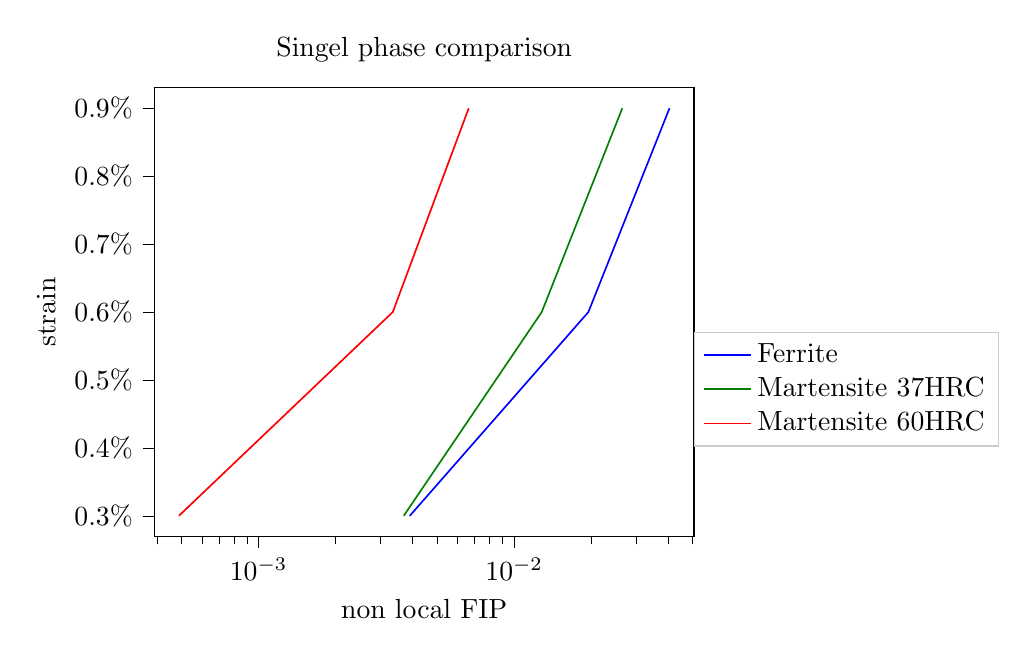
\begin{tikzpicture}

\begin{axis}[
legend cell align={left},
legend style={
  fill opacity=0.8,
  draw opacity=1,
  text opacity=1,
  at={(1,0.2)},
  anchor=south west,
  draw=white!80!black
},
log basis x={10},
tick align=outside,
tick pos=left,
title={Singel phase comparison},
x grid style={white!69.0196078431373!black},
xlabel={non local FIP},
xmin=0.000391210977939241, xmax=0.0505797014692806,
xmode=log,
xtick style={color=black},
y grid style={white!69.0196078431373!black},
ylabel={strain},
ymin=0.27, ymax=0.93,
ytick style={color=black},
ytick={0.2,0.3,0.4,0.5,0.6,0.7,0.8,0.9,1},
yticklabels={0.2\%,0.3\%,0.4\%,0.5\%,0.6\%,0.7\%,0.8\%,0.9\%,1.0\%}
]
\addplot [semithick, blue]
table {%
0.00390741510966807 0.3
0.019531057737275 0.6
0.0405504823068248 0.9
};
\addlegendentry{Ferrite}
\addplot [semithick, green!50!black]
table {%
0.00369963690382581 0.3
0.0128257416304683 0.6
0.0264986952067736 0.9
};
\addlegendentry{Martensite 37HRC}
\addplot [semithick, red]
table {%
0.00048796791924573 0.3
0.00335206561369479 0.6
0.00664282169547196 0.9
};
\addlegendentry{Martensite 60HRC}
\end{axis}

\end{tikzpicture}
